\chapterquote{You're a wizard, Harry.}{Harry Potter and the Philosopher's Stone}

There's only one theorem, so this will be a short chapter. The only prerequisites are angle chasing theorems in circles.

\section{Power of a Point}

The Power of a Point theorem helps us length chase in circles. The proof is a result of similar triangles, and its uses are numerous in lower-level competitions. If you already know this theorem, feel free to skip this section.

\begin{theo}[Power of a Point]
Let line $\ell_1$ intersect circle $\omega$ at $A,B$ line $\ell_2$ intersect $\omega$ at $C,D,$ and $\ell_1$ intersect $\ell_2$ at $P.$ Then $PA\cdot PB=PC\cdot PD.$
\end{theo}

\begin{pro}
There are two cases here: Either $P$ is inside of $\omega$ or outside of $\omega.$

If $P$ is inside of $\omega,$ then note that by Inscribed Angle, $\angle PAC=\angle PDB$ and $\angle=\angle PAB,$ so $\triangle PAC\sim \triangle PDB.$

If $P$ is outside of $\omega,$ then without loss of generality, let $PA\leq PB$ and $PC\leq PD.$ Then note $\angle PAC=180^{\circ}-\angle CAB=\angle PDB$ and $\angle PCA=180^{\circ}-\angle ACD=\angle PBD,$ so $\triangle PAC\sim\triangle PDB.$

To finish, note that the similarity implies $\frac{PA}{PC}=\frac{PD}{PB}$, or $PA\cdot PB=PC\cdot PB.$

\begin{center}
\begin{asy}
size(4cm);
//Generated By AsyPadv1.2
import olympiad;
import markers;
import math;
import graph;

//colored pens
pen c000000 = rgb("000000");
//dependency level 0
/* You can change the coordinates of these points of dependency level 0.
The drawing will retain the same relationships and qualities.
Please be aware that as a result of this some of the image may be clipped off. */
pair A = (4.72, 17.13); dot(A, c000000); label("$A$", A, dir(136.636577041617));
pair B = (4.38, 16.06); dot(B, c000000); label("$D$", B, dir(236.09372301155847));
pair C = (6.13, 15.99); dot(C, c000000); label("$B$", C, dir(319.3987053549977));
//dependency level 1
//Do not change anything below, unless you are experienced in Asymptote.
path ccA_B_C = circumcircle(A, B, C);
pair ccA_B_Ccenter = circumcenter(A, B, C); real ccA_B_Crad = circumradius(A, B, C); draw(ccA_B_C, c000000);
path segA_C = A--C; draw(segA_C, c000000);
//dependency level 2
pair D = relpoint(ccA_B_C, 0.1252472145174768); dot(D, c000000); label("$C$", D, dir(48.14541204060811));
//dependency level 3
path segB_D = B--D; draw(segB_D, c000000);
//dependency level 4
pair P = intersectionpoint(segA_C, segB_D); dot(P, c000000); label("$P$", P, dir(79.06275557490466));
\end{asy}
\begin{asy}
//Generated By AsyPadv1.2
import olympiad;
import markers;
import math;
import graph;
//change the unit size to fit your needs
size(4cm);
//colored pens
pen c000000 = rgb("000000");
//dependency level 0
/* You can change the coordinates of these points of dependency level 0.
The drawing will retain the same relationships and qualities.
Please be aware that as a result of this some of the image may be clipped off. */
pair A = (3.47, 17.85); dot(A, c000000); label("$A$", A, dir(126.02737338510292));
pair B = (2.88, 16.31); dot(B, c000000); label("$B$", B, dir(236.09372301155847));
pair C = (4.64, 16.25); dot(C, c000000); label("$C$", C, dir(319.3987053549977));
//dependency level 1
//Do not change anything below, unless you are experienced in Asymptote.
path ccA_B_C = circumcircle(A, B, C);
pair ccA_B_Ccenter = circumcenter(A, B, C); real ccA_B_Crad = circumradius(A, B, C); draw(ccA_B_C, c000000);
path lineB_A = (B-20.0*unit(A-B))--(A+20.0*unit(A-B)); 
//dependency level 2
pair D = relpoint(ccA_B_C, 0.21889966793444027); dot(D, c000000); label("$D$", D, dir(48.14541204060811));
//dependency level 3
path lineD_C = (D-20.0*unit(C-D))--(C+20.0*unit(C-D)); 
//dependency level 4
pair P = intersectionpoint(lineB_A, lineD_C); dot(P, c000000); label("$P$", P, dir(84.11889062937553));
//dependency level 5
path segP_B = P--B; draw(segP_B, c000000);
path segP_C = P--C; draw(segP_C, c000000);
\end{asy}

\textit{$P$ inside $\omega$ and $P$ outside $\omega.$}
\end{center}
\end{pro}

In the case of tangency, $A=B$ is the point of tangency. (You can think of a tangent line intersecting a circle twice at the same point.)

The Two Tangent Theorem is a corollary of Power of a Point. It states that the lengths of the two tangents from a point to a circle are equal.

\begin{fact}[Two Tangent Lemma]
Let the tangents from point $P$ to circle $\omega$ intersect $\omega$ at $A,B.$ Then $PA=PB.$
\begin{hint}
\begin{addhint}
{Use power of a point to relate $PA$ and $PB.$}
\end{addhint}
\end{hint}
\begin{solu}
\begin{addsol}
{Note that by Power of a Point, $PA^2=PB^2.$

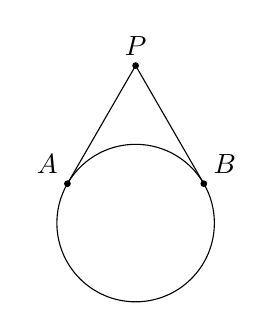
\begin{tikzpicture}
\draw (-0.8660254037844386,0.5)--(0,2)--(0.8660254037844386,0.5);
\draw (0,0) circle (1);
\filldraw (-0.8660254037844386,0.5) circle (1pt) node[anchor=south east] {$A$};
\filldraw (0.8660254037844386,0.5) circle (1pt) node[anchor=south west] {$B$};
\filldraw (0,2) circle (1pt) node[anchor=south] {$P$};
\end{tikzpicture}}
\end{addsol}
\end{solu}
\end{fact}

\section{Bisector Lemma}

This is a very powerful fact that kills a lot of earlier computational geometry problems involving circles.

\begin{fact}[Bisector Lemma]
Let $\omega_1$ and $\omega_2$ intersect at $X$ and $Y,$ and let $\ell$ be a line tangent to $\omega_1$ and $\omega_2.$ If $\ell$ intersects $\omega_1$ at $A$ and $\omega_2$ at $B,$ then $XY$ bisects $AB.$
\end{fact}

\begin{pro}
Let $XY$ intersect $AB$ at $P.$ Then by Power of a Point, $PX^2=PA\cdot PB=PY^2.$
\begin{center}
\begin{asy}
size(6cm);
real xmin = -4.5, xmax = 4, ymin = -3, ymax = 35;

draw(circle((-2,0), 2.23606797749979)); 
draw(circle((1,0), 2.8284271247461903)); 
draw((xmin, 0.20141850719855647*xmin + 2.68381204170681)--(xmax, 0.20141850719855647*xmax + 2.68381204170681)); /* line */
draw((-1,2.4823935345082537)--(-1,-2)); 

dot("$X$",(-1,2),dir(5));
dot("$Y$",(-1,-2),dir(55));
dot("$A$",(-2.4415184401122536,2.1920450422016526),dir(100)); 
dot("$B$",(0.44151844011225216,2.7727420268148544),dir(100)); 
dot("$P$",(-1,2.4823935345082537),dir(100)); 
clip((xmin,ymin)--(xmin,ymax)--(xmax,ymax)--(xmax,ymin)--cycle); 
\end{asy}
\end{center}
\end{pro}

\section{Summary}

\subsection{Theory}

\begin{enumerate}
\item Power of a Point
\begin{itemize}
\Item If lines $\ell_1,\ell_2$ through $P$ intersect circle $\omega$ at $A,B$ and $C,D,$ respectively, then $PA\cdot PB=PC\cdot PD.$

\Item This is a consequence of similar triangles.
\end{itemize}
\item Bisector Lemma
\begin{itemize}
\Item The common chord of two circles bisects the common external tangent.
\end{itemize}
\end{enumerate}

\subsection{Tips and Strategies}

\begin{enumerate}
\item If there are two circles and you're in doubt, use Bisector Lemma. (This even applies for some easier olympiad problems.)
\end{enumerate}

\pagebreak

\section{Exercises}

\subsection{Check-ins}

\begin{enumerate}
\item Let chords $AB$ and $CD$ in circle $\omega$ intersect at $P.$ If $AP=BP=4$ and $CP=2,$ find $DP.$

\begin{asy}
//Generated By AsyPadv1.2
import olympiad;
import markers;
import math;
import graph;
//change the unit size to fit your needs
size(3cm);
//colored pens
pen c000000 = rgb("000000");
//dependency level 0
/* You can change the coordinates of these points of dependency level 0.
The drawing will retain the same relationships and qualities.
Please be aware that as a result of this some of the image may be clipped off. */
pair A = (3.32, 17.11); dot(A, c000000); label("$A$", A, dir(207.8972710309471));
pair B = (5.05, 17.09); dot(B, c000000); label("$B$", B, dir(325.00797980144));
//dependency level 1
//Do not change anything below, unless you are experienced in Asymptote.
path pbA_B = ((A+B)/2-20.0*unit(((B-A).y, -(B-A).x)))--((A+B)/2+20.0*unit(((B-A).y, -(B-A).x))); 
path segA_B = A--B; draw(segA_B, c000000);
//dependency level 2
pair C = relpoint(pbA_B, 0.5134646278119219); dot(C, c000000); label("$C$", C, dir(274.31287501714553));
pair P = intersectionpoint(pbA_B, segA_B); dot(P, c000000); label("$P$", P, dir(50.95410743116071));
//dependency level 3
path ccA_C_B = circumcircle(A, C, B);
pair ccA_C_Bcenter = circumcenter(A, C, B); real ccA_C_Brad = circumradius(A, C, B); draw(ccA_C_B, c000000);
//dependency level 4
pair D = intersectionpoints(pbA_B, ccA_C_B)[0]; dot(D, c000000); label("$D$", D, dir(88.75312672365999));
//dependency level 5
path segD_C = D--C; draw(segD_C, c000000);
\end{asy}

\item Let the tangent through $A$ to circle $\omega$ intersect line $\ell$ that passes through $B,C$ on $\omega$ at $P.$ If $BP<CP,$ $AP=4,$ and $BC=6,$ find $BP.$

\begin{asy}
import olympiad;
import markers;
import math;
import graph;
//change the unit size to fit your needs
size(3cm);
//colored pens
pen c000000 = rgb("000000");
//dependency level 0
/* You can change the coordinates of these points of dependency level 0.
The drawing will retain the same relationships and qualities.
Please be aware that as a result of this some of the image may be clipped off. */
pair C = (4.51, 16.84); dot(C, c000000); label("$C$", C, dir(25.70995378080977));
pair D = (3.19, 16.32); 
pair P = (2.25, 18.25); dot(P, c000000); label("$P$", P, dir(91.48786752882734));
//dependency level 1
//Do not change anything below, unless you are experienced in Asymptote.
path circD_C = Circle(D, abs(D-C));
pair circD_Ccenter = D; real circD_Crad = abs(D - C); draw(circD_C, c000000);
path segP_C = P--C; draw(segP_C, c000000);
//dependency level 2
pair P_circD_C_tangent1 = tangent(P, circD_Ccenter, circD_Crad, 1);
path tl1P_circD_C = (P-20.0*unit(P_circD_C_tangent1-P))--(P_circD_C_tangent1+20.0*unit(P_circD_C_tangent1-P)); 
pair B = intersectionpoints(segP_C, circD_C)[0]; dot(B, c000000); label("$B$", B, dir(81.55446702351315));
//dependency level 3
pair A = tangent(P,circD_Ccenter, circD_Crad,1);
dot("$A$", A, dir(155.9863895131953));
//dependency level 4
path segP_A = P--A; draw(segP_A, c000000);
\end{asy}

\item Let line $\ell_1$ that passes through $A,B$ on circle $\omega$ intersect line $\ell_2$ that passes through $C,D$ on $\omega$ at $P.$ If $PA=6,$ $AB=12,$ and $PC=3,$ find $CD.$

\begin{asy}
//Generated By AsyPadv1.2
import olympiad;
import markers;
import math;
import graph;
//change the unit size to fit your needs
size(3cm);
//colored pens
pen c000000 = rgb("000000");
//dependency level 0
/* You can change the coordinates of these points of dependency level 0.
The drawing will retain the same relationships and qualities.
Please be aware that as a result of this some of the image may be clipped off. */
pair D = (4.25, 16.81); dot(D, c000000); label("$D$", D, dir(25.70995378080977));
pair O = (3.19, 16.32); 
pair P = (2.71, 17.84); dot(P, c000000); label("$P$", P, dir(91.48786752882734));
//dependency level 1
//Do not change anything below, unless you are experienced in Asymptote.
path circO_D = Circle(O, abs(O-D));
pair circO_Dcenter = O; real circO_Drad = abs(O - D); draw(circO_D, c000000);
path segP_D = P--D; draw(segP_D, c000000);
//dependency level 2
pair C = intersectionpoints(segP_D, circO_D)[0]; dot(C, c000000); label("$C$", C, dir(81.55446702351315));
pair B = relpoint(circO_D, -0.4892866639289171); dot(B, c000000); label("$B$", B, dir(315.0));
//dependency level 3
path segP_B = P--B; draw(segP_B, c000000);
//dependency level 4
pair A = intersectionpoints(segP_B, circO_D)[0]; dot(A, c000000); label("$A$", A, dir(315.0));
\end{asy}

\item Let $\triangle ABC$ have a right angle at $C$ and let $P$ be the foot of the altitude from $C$ to $AB.$ If the foot of the altitude from $P$ to $AC$ is $X$ and the foot from $P$ to $BC$ is $Y,$ then prove that $AXYB$ is cyclic.
\end{enumerate}

\subsection{Problems}

\begin{enumerate}
\item Let $PA$ and $PB$ be tangents to circle $\omega,$ and let line $\ell$ through $P$ intersect $\omega$ at $X$ and $C$ and $AB$ at $Y.$ If $PA=4$, $PC=8,$ $AY=1$, and $XY=1,$ find the area of $\triangle PAB.$

\begin{asy}
//Generated By AsyPadv1.2
import olympiad;
import markers;
import math;
import graph;
//change the unit size to fit your needs
size(6cm);
//colored pens
pen c000000 = rgb("000000");
//dependency level 0
/* You can change the coordinates of these points of dependency level 0.
The drawing will retain the same relationships and qualities.
Please be aware that as a result of this some of the image may be clipped off. */
pair B = (3.88, 17.20); dot(B, c000000); label("$B$", B, dir(51.60483549675433));
pair O = (3.19, 16.32); 
//dependency level 1
//Do not change anything below, unless you are experienced in Asymptote.
path circO_B = Circle(O, abs(O-B));
pair circO_Bcenter = O; real circO_Brad = abs(O - B); draw(circO_B, c000000);
path segO_B = O--B; 
//dependency level 2
pair C = relpoint(circO_B, -0.3326246702692839); dot(C, c000000); label("$C$", C, dir(253.50839790887915));
pair A = relpoint(circO_B, -0.6270403362062634); dot(A, c000000); label("$A$", A, dir(120.96189753921033));
path perB_segO_B = (B-20.0*(dir(segO_B).y, -dir(segO_B).x))--(B+20.0*(dir(segO_B).y, -dir(segO_B).x)); 
//dependency level 3
path segA_O = A--O; 
path segA_B = A--B; draw(segA_B, c000000);
//dependency level 4
path perA_segA_O = (A-20.0*(dir(segA_O).y, -dir(segA_O).x))--(A+20.0*(dir(segA_O).y, -dir(segA_O).x)); 
//dependency level 5
pair P = intersectionpoint(perA_segA_O, perB_segO_B); dot(P, c000000); label("$P$", P, dir(88.28051995968144));
//dependency level 6
path segP_C = P--C; draw(segP_C, c000000);
path segP_A = P--A; draw(segP_A, c000000);
path segP_B = P--B; draw(segP_B, c000000);
//dependency level 7
pair X = intersectionpoints(segP_C, circO_B)[0]; dot(X, c000000); label("$X$", X, dir(129.2296640975739));
pair Y = intersectionpoint(segA_B, segP_C); dot(Y, c000000); label("$Y$", Y, dir(133.61835402638553));
//clip the drawing view
clip((0.0, 13.0)--(0.0, 20.0)--(10.0, 20.0)--(10.0, 13.0)--cycle);
\end{asy}


\item Consider two externally tangent circles $\omega_1,\omega_2.$ Let them have common external tangents $AC,BD$ such that $A,B$ are on $\omega_1$ and $C,D$ are on $\omega_2.$ Let $AC$ intersect $BD$ at $P,$ and let the common internal tangent intersect $AC$ and $BD$ at $X$ and $Y$. If $\frac{[PCD]}{[PAB]}=\frac{1}{25},$ find $\frac{[PCD]}{[PXY]}.$

\item (Mandelbrot 2012) Let $A$ and $B$ be points on the lines $y=3$ and $y=12,$ respectively. There are two circles passing through $A$ and $B$ that are also tangent to the $x$ axis, say at $P$ and $Q.$ Suppose that $PQ=2012.$ Find $AB.$

\item (Parody) Consider a coordinate plane with two circles tangent to the $x$ axis at $X,Y,$ respectively. If the circles intersect at $P,Q,$ and $XY=8,$ is it possible for $P$ to lie on $y=3$ and $Q$ to lie on $y=12?$

\item (e-dchen Mock MATHCOUNTS) Consider chord $AB$ of circle $\omega$ centered at $O.$ Let $P$ be a point on segment $AB$ such that $AP=2$ and $BP=8$. If $\angle APO=150^{\circ},$ what is the area of $\omega?$
\end{enumerate}

\section{Challenges}

\begin{enumerate}
	\item (Geometry Bee 2019) Circles $O_1$ and $O_2$ are constructed with $O_1$ having radius of $2,$ $O_2$ having radius of $4,$ and $O_2$ passing through the point $O_1.$ Lines $\ell_1$ and $\ell_2$ are drawn so they are tangent to both $O_1$ and $O_2.$ Let $O_1$ and $O_2$ intersect at points $P$ and $Q.$ Segment $\overline{EF}$ is drawn through $P$ and $Q$ such that $E$ lies on $\ell_1$ and $F$ lies on $\ell_2.$ What is the length of $\overline{EF}?$
	
\item (AMC 10B 2013/23) In triangle $ABC$, $AB=13$, $BC=14$, and $CA=15$. Distinct points $D$, $E$, and $F$ lie on segments $\overline{BC}$, $\overline{CA}$, and $\overline{DE}$, respectively, such that $\overline{AD}\perp\overline{BC}$, $\overline{DE}\perp\overline{AC}$, and $\overline{AF}\perp\overline{BF}$. The length of segment $\overline{DF}$ can be written as $\frac{m}{n}$, where $m$ and $n$ are relatively prime positive integers. What is $m+n$?
\begin{solu}
\begin{addsol}
{Let the circle with diameter $AB$ be $\omega.$ Note $\omega$ intersects $DE$ at $D,F$ and $AC$ at $H$ where $H$ is the foot of the altitude from $B$ to $AC.$

Now note $EF\cdot ED=EH\cdot EA,$ or $EF\cdot \frac{36}{5}=3\cdot \frac{48}{5}.$ So $EF=4$ and $DF=\frac{16}{5},$ so the answer is $21.$}
\end{addsol}
\end{solu}
\end{enumerate}